Les recherches menées lors de mon premier postdoc au MSSMat portait sur le contrôle non-destructif \textit{in situ} des matériaux polycristallins.
Dans ce contexte, les techniques utilisant les ultrasons sont couramment utilisées dans l'industrie.
Ces dernière reposent sur l'atténuation du signal résultant de l'interaction entre les ondes et hétérogénéités constitutives entre les grains.
Il est en effet possible de relier la perte d'amplitude d'un signal s'étant propagé dans un polycristal, quantifiée par le coefficient d'atténuation $\alpha$, à une mesure moyenne de la taille des grains présents dans l'échantillon \cite{stanke}.
Ainsi, une bonne connaissance des mécanismes d'atténuation et de diffusion des ondes ultrasonores permet de remonter à certaines informations sur la microstructure.


\paragraph{Motivations:}
$\newline$
Les développements théoriques mentionnés sont bien adaptés pour des microstructures dont la taille des grains est relativement homogène, c'est à dire une distribution avec un faible écart-type.
En revanche, la caractérisation de distributions de taille de grain plus \textit{étalées} peut être améliorée.
L'objectif de ces travaux est de proposer une approche de caractérisation expérimentale des distributions bimodales de taille de grain (\textit{i.e. un mélange de ``gros'' et de ``petits'' grains}).
D'un côté, ces dernières représentent un intérêt pour les propriétés chimiques ou mécaniques qu'elles peuvent conférer au matériau \cite{Chakrabarti2009_bimodal,Sabzi2016_bimodal}, de l'autre, cette étude constitue un premier pas vers la caractérisation de distributions à fort écart-type pouvant être approximées par des distributions multimodales.

% On s'intéresse ici au contrôle non-destructif par ultrasons, couramment utilisé dans l'industrie pour la caractérisation de microstructures polycristallines.
% Ces techniques reposent sur le fait qu'en se propageant dans un polycristal, les ondes ultrasonores sont continuellement atténuées et dispersées par les hétérogénéités constitutives entre les grains.
%Il est par exemple possible de relier la perte d'amplitude d'un signal s'étant propagé dans un polycristal, quantifiée par le coefficient d'atténuation $\alpha$, à une mesure moyenne de la taille des grains présents dans l'échantillon \cite{stanke}.

% La simulation numérique est un outil permettant une mise en évidence et une meilleure compréhension des phénomènes à l'\oe uvre, qui peuvent aider à déduire du signal ultrasonore plus d'informations sur la microstructure.  


\paragraph{Contributions:}
$\newline$
Dans ces travaux, la simulation numérique se substitue aux essais \textit{in situ}.
On s'appuie alors sur une librairie de calcul parallèle par éléments finis développée en C++ au MSSMat \cite{TIE2018} et basée sur la formulation DG.
Ma première tâche était  d'étendre l'implémentation aux problèmes tridimensionnels et à l'utilisation de géométries provenant du logiciel \textsc{Neper} \cite{Neper}.
\textsc{Neper} permet de générer (i) des microstructures morphologiquement réalistes par tessellation/optimisation; (ii) des orientations cristallographiques qui déterminent le comportement élastique orthotrope des grains.
La figure \ref{subfig:microstructure} montre un exemple de microstructure de morphologie ``croissance de grain'' de diamètre équivalent moyen $\left\langle d \right\rangle = 460 \mu m$, provenant du logiciel. %dont le diamètre équivalent des grains suit une loi lognormale $$de moyenne $\mu=460 \mu m$ et d'écart-type $\sigma = 0.03$, provenant du logiciel.

En suivant la procédure de calcul développée dans une thèse effectuée au laboratoire \cite{Bai2018-noise}, un problème d'onde plane est résolu numériquement dans la microstructure (voir figure \ref{subfig:ondePlane}) et dans le milieu homogène équivalent.
\begin{figure}[h!]
  \centering
  \subcaptionbox{Microstructure \label{subfig:microstructure}}{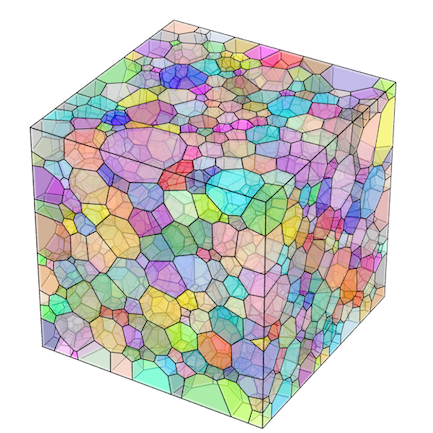
\includegraphics[height=0.4\textwidth]{pngFigures/cube460mm_100x100_croped.png}}
  \subcaptionbox{Onde plane incidente \label{subfig:ondePlane}}{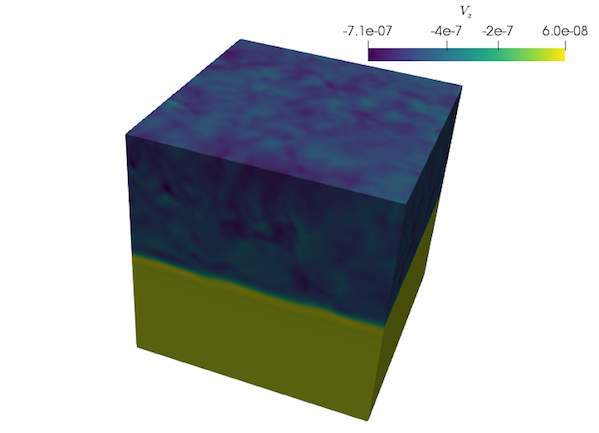
\includegraphics[height=0.4\textwidth]{pngFigures/velocity_100_croped.png}}
  % \caption{(\subref{subfig:microstructure}) Exemple de microstructure générée avec le logiciel \textsc{Neper} -- (\subref{subfig:ondePlane}) propagation d'une onde plane dans la microstructure \subref{subfig:microstructure}.}
  \caption{Exemple de microstructure générée avec le logiciel \textsc{Neper} et effet de l'anisotropie et de l'hétérogénéité des propriétés mécaniques sur la propagation d'une onde plane.}
  \label{fig:microStruct}
\end{figure}
%% chargement à spectre large
Les solutions en déplacement et vitesse calculées pour chaque milieu sur la face chargée ou sur la face opposée sont ensuite passées dans le domaine fréquentiel et comparées de sorte à tracer des courbes d'évolution du coefficient $\alpha$ en fonction de la fréquence.

Sur le plan théorique, on montre que le coefficient d'atténuation peut être exprimé pour les microstructures bimodales comme une somme de contributions provenant de chaque famille de grains.
Ces dernières étant pondérées par la fraction volumique correspondante.
Les résultats numériques obtenus sont en accord avec cette propriétés, comme en témoignent les courbes de la figure \ref{fig:attenuation}.
Ces courbes résultent de calculs théoriques et numériques dans une microstructure bidimensionnelle comportant deux tailles de grains caractérisées par les diamètres équivalents $\left\langle d \right\rangle =\{80,240\} \: \mu m$.
Les différences observables entre les figures \ref{fig:test} et \ref{fig:test_num} s'expliquent par le fait que la théorie est basée sur l'hypothèse de diffusion simple des ondes (\textit{i.e. une seule réflexion des ondes}), tandis que la modélisation numérique prend en compte la diffusion multiple. 
On voit qu'à mesure que la fraction volumique de gros grains $F_{GG}$ décroit (\textit{resp. augmente}), la courbe d'atténuation se rapproche du cas d'une microstructure monomodale constituée uniquement de petits (\textit{resp. gros}) grains.
%%
% Les premiers résultats numériques obtenus montrent que lorsque la distribution de diamètre équivalent dans la microstructure est bimodale, les courbes $\alpha(f)$ et $\beta(f)$ changent avec la fraction volumique de gros grains (FGG).
% La figure \ref{fig:attenuation} illustre ce dernier point pour l'atténuation sur un cas bidimensionnel dans lequel les deux tailles de grain considérées sont $\left\langle d \right\rangle =\{80,240\} \: \mu m$.
\begin{figure}[h!]
  \centering
  {\phantomsubcaption{\label{fig:test}}}
  {\phantomsubcaption{\label{fig:test_num}}}
  \begin{tikzpicture}% ,yticklabels at=edge left,ylabels at=edge left
  \begin{groupplot}[group style={group size=2 by 1,horizontal sep=3ex,vertical sep=1ex,yticklabels at=edge left,ylabels at=edge left,xticklabels at=edge bottom,xlabels at=edge bottom}
    % ,ymajorgrids=true,xmajorgrids=true,axis on top%,scale only axis,
    ,width=0.5\textwidth
    ,xlabel=$f$(MHz),ylabel=$\alpha$(1/m)
    ,ymin=0,xmin=0
    %,xmax=20
    ,ymax=140
    % ,ymax=220
    ]
    
    
    \nextgroupplot[title={(a) Théorique}]
    %% 240-80
    
    
    \addplot[black!50,thick] table[x expr=\thisrow{f}/1.e6,y=80mm] {pgfFigures/pgfFiles/bimodal_analytical2D.pgf};
    \addplot[black,thick] table[x expr=\thisrow{f}/1.e6,y=240mm] {pgfFigures/pgfFiles/bimodal_analytical2D.pgf};

    % \addplot[Blue,only marks,mark repeat=3,mark=+,thick] table[x expr=\thisrow{f}/1.e6,y=240_80mm_25] {pgfFigures/pgfFiles/bimodal_analytical2D.pgf};
    \addplot[Blue,thick,densely dotted] table[x expr=\thisrow{f}/1.e6,y expr=0.75*\thisrow{80mm}+0.25*\thisrow{240mm}] {pgfFigures/pgfFiles/bimodal_analytical2D.pgf};

    % \addplot[Green,only marks,mark repeat=3,mark=x,thick] table[x expr=\thisrow{f}/1.e6,y=240_80mm_50] {pgfFigures/pgfFiles/bimodal_analytical2D.pgf};
    \addplot[Green,thick] table[x expr=\thisrow{f}/1.e6,y expr=0.5*\thisrow{80mm}+0.5*\thisrow{240mm}] {pgfFigures/pgfFiles/bimodal_analytical2D.pgf};

    %\addplot[Red,only marks,mark repeat=3,mark=asterisk,thick] table[x expr=\thisrow{f}/1.e6,y=240_80mm_75] {pgfFigures/pgfFiles/bimodal_analytical2D.pgf};
    \addplot[Red,thick, dashed] table[x expr=\thisrow{f}/1.e6,y expr=0.25*\thisrow{80mm}+0.75*\thisrow{240mm}] {pgfFigures/pgfFiles/bimodal_analytical2D.pgf};

    % \node[right,Red] at (15,68) {\scriptsize $\epsilon=3\%$};
    % \node[right,Green] at (15,84.2) {\scriptsize $\epsilon=4\%$};
    % \node[right,Blue] at (15,103.52) {\scriptsize $\epsilon=2\%$};

    
    \nextgroupplot[title={(b) Numérique},legend style={at={($(.75,-0.3)+(0.5cm,0.35cm)$)},legend columns=5}]
    %% 160-80

    \addplot[black!50,thick] table[x expr=\thisrow{f}/1.e6,y=FLG0] {pgfFigures/pgfFiles/bimodal160_80_2D.pgf};
    \addplot[black,thick] table[x expr=\thisrow{f}/1.e6,y=FLG100] {pgfFigures/pgfFiles/bimodal240_160_2D.pgf};

    \addplot[Blue,thick,densely dotted] table[x expr=\thisrow{f}/1.e6,y=FLG25] {pgfFigures/pgfFiles/bimodal240_80_2D.pgf};
    
    \addplot[Green,thick] table[x expr=\thisrow{f}/1.e6,y=FLG50] {pgfFigures/pgfFiles/bimodal240_80_2D.pgf};
    
    \addplot[Red,thick,dashed] table[x expr=\thisrow{f}/1.e6,y=FLG75] {pgfFigures/pgfFiles/bimodal240_80_2D.pgf};
    


    \addlegendentry{ $F_{GG}=0$}
    \addlegendentry{ $F_{GG}=1$}

    \addlegendentry{ $F_{GG}=0.25$}
    % \addlegendentry{$\alpha_{Th}$ $F_{GG}=0.25$}
    % \addlegendentry{Expected $F_{GG}=0.25$}

    \addlegendentry{ $F_{GG}=0.50$}
    % \addlegendentry{$\alpha_{Th}$ $F_{GG}=0.50$}
    % \addlegendentry{Expected $F_{GG}=0.50$}

    \addlegendentry{ $F_{GG}=0.75$}
    %\addlegendentry{$\alpha_{Th}$ $F_{GG}=0.75$}
    %\addlegendentry{Expected $F_{GG}=0.75$}

    
  \end{groupplot}
\end{tikzpicture}



%%% Local Variables:
%%% mode: latex
%%% TeX-master: "../manuscript"
%%% End:

  \caption{{\'E}volution du coefficient d'atténuation en fonction de la fréquence pour des microstructures 2D unimodales et bimodales: comparaison entre les prédictions théoriques et les résultats numériques. L'influence de la Fraction volumique de Gros Grains ($F_{GG}$) est mise en évidence.}
  \label{fig:attenuation}
\end{figure}
% En particulier, les courbes semblent tendre vers celles des deux distributions unimodales pour les cas limites $FGG \rightarrow 0$ et $FGG \rightarrow 100 \%$.

%En appliquant la procédure à différentes microstructures (bi- ou tridimensionnelles, avec ou sans concentration de gros grains dans certaines régions, \textit{etc.}), l'idée est de déduire un maximum d'informations des courbes $\alpha(f)$ et $\beta(f)$ par comparaison avec le modèle unimodal.

{\`A} partir de ces résultats, une procédure de caractérisation des distributions bimodales de la taille de grain a été proposée.
Elle consiste, à partir d'une courbe d'atténuation obtenue sur une microstructure, à résoudre un problème d'optimisation à trois paramètres basé sur les prédictions théoriques monomodales.
Les trois paramètres étant la fraction volumique de gros grains, le diamètre équivalent moyen des gros grains et celui des petits grains, les microstructures bimodales peuvent être caractérisées.
Cette approche conduit à des résultats satisfaisants pour peu que les courbes monomodales utilisées comme référence dans le problème d'optimisation soient bien représentatives de la réalité.
On peut donc imaginer utiliser un grand nombre de courbes d'atténuation expérimentales pour un matériau donné afin d'\textit{alimenter} le problème d'optimisation et obtenir des caractérisation de plus en plus précises.
Ceci ne constitue toutefois pour l'instant qu'une perspective de ces travaux.

\paragraph{Publication associée:}
$\newline$ 
\begin{itemize}
\item A. Renaud, B. Tie, J.H Schmitt and A.S. Mouronval, ``Multi-parameter optimization of attenuation data for characterizing grain size distributions and application to bimodal microstructures'', Ultrasonics, \textit{Soumis le 21/11/20 -- révision mineure requise le 16/02/21}
\end{itemize}




%%% Local Variables:
%%% mode: latex
%%% TeX-master: "main"
%%% End:
